% !TEX encoding = UTF-8
% !TEX TS-program = pdflatex
% !TEX root = relazione.tex
% !TEX spellcheck = it-IT
\documentclass[12pt, a4paper,titlepage]{article}
\usepackage[italian]{babel}
\usepackage[utf8]{inputenc}
\usepackage{graphicx}
\usepackage[tc]{titlepic}
\usepackage{eurosym}
\usepackage{epstopdf}
\usepackage{pdflscape}
\usepackage[margin=2.5cm]{geometry}
\usepackage{float}
\usepackage{listings}
\usepackage[usenames,dvipsnames]{color}
\usepackage{hyperref}
\hypersetup{
    colorlinks=true,
    linkcolor=black
}
\usepackage{booktabs}
\graphicspath{{./pic/}}
\usepackage{fancyhdr}% http://ctan.org/pkg/fancyhdr
\usepackage{lastpage}
\usepackage{pifont}
\newcommand{\cmark}{\ding{51}}%
\newcommand{\xmark}{\ding{55}}%
\fancyhf{}% Clear header/footer
\fancyfoot[L]{\slshape\rightmark}
\fancyfoot[R]{Pag. \thepage\ di \pageref{LastPage}}% \fancyfoot[R]{\thepage}
\renewcommand{\headrulewidth}{0pt}% Default \headrulewidth is 0.4pt
\renewcommand{\footrulewidth}{0.4pt}% Default \footrulewidth is 0pt
\usepackage{letltxmacro}
\usepackage{pgffor}


%% https://tex.stackexchange.com/questions/14393/how-keep-a-running-list-of-strings-and-then-process-them-one-at-a-time
\newcommand\FigList{}
\newcommand\AddFigToList[1]{\edef\FigList{\FigList#1,}}

\LetLtxMacro{\OldIncludegraphics}{\includegraphics}
\renewcommand{\includegraphics}[2][]{%
    \AddFigToList{#2}%
    \OldIncludegraphics[#1]{#2}%
}

\newcommand*{\ShowListOfFigures}{%
    \typeout{Figures included were}%
    \foreach \x in \FigList {%
        %\par\x% <-- uncomment if you want the list in the PDF as well
        \typeout{ \x}
    }%
}
\AtEndDocument{\ShowListOfFigures}

%fine impostazioni
\begin{document}
\begin{titlepage}

\newcommand{\HRule}{\rule{\linewidth}{0.5mm}} % Defines a new command for the horizontal lines, change thickness here

\center % Center everything on the page

%----------------------------------------------------------------------------------------
% HEADING SECTIONS
%----------------------------------------------------------------------------------------

\vspace*{\fill}
\textsc{\Large Università degli Studi di Padova}\\[0.5cm] % Major heading such as course name
\textsc{\large Corso di Laurea Magistrale in Informatica}\\[0.5cm] % Minor heading such as course title

%----------------------------------------------------------------------------------------
% TITLE SECTION
%----------------------------------------------------------------------------------------

\HRule \\[0.4cm]
{ \huge \textbf{Web Information Management}\\[0.4cm] Analisi di usabilità di NintendoLife.com}\\[0.4cm] % Title of your document
\HRule \\[0.5cm]
\large{Anno Accademico 2016/2017}\\[1cm]

\includegraphics[scale=0.3]{logo}\\[1cm] % Include a department/university logo - this will require the graphicx package
%----------------------------------------------------------------------------------------
% AUTHOR SECTION
%----------------------------------------------------------------------------------------
Jacopo Cavallarin, 1131015
\vspace*{\fill}
% If you don't want a supervisor, uncomment the two lines below and remove the section above
%\Large \emph{Author:}\\
%John \textsc{Smith}\\[3cm] % Your name

%----------------------------------------------------------------------------------------
% LOGO SECTION
%----------------------------------------------------------------------------------------



%----------------------------------------------------------------------------------------

\vfill % Fill the rest of the page with whitespace

\end{titlepage}
\newpage
\tableofcontents
%\listoffigures
\thispagestyle{empty}
\clearpage
\pagenumbering{arabic}
\pagestyle{fancy}

\section{Introduzione}
\label{sec:introduzione}
\subsection{Descrizione del sito in esame}
\begin{figure}[h]
\centering

\includegraphics[width=.5\textwidth]{Logo_sito}
\end{figure}
URL completa del sito: \url{http://www.nintendolife.com}\\
NintendoLife è un sito che raccoglie tutte le novità riguardanti i prodotti di Nintendo, la famosa azienda giapponese di videogiochi. Oltre a riportare le ultime notizie, il sito propone recensioni e anteprime (spesso accompagnate da video) dei principali titoli prodotti per le console Nintendo e dei titoli per smartphone prodotti da Nintendo.\\
Oltre agli articoli, il sito contiene un forum a cui gli utenti possono registrarsi per discutere su ogni cosa che riguarda il mondo Nintendo.
\subsection{Periodo di analisi}
L'analisi del sito è stata effettuata durante il mese di Maggio 2017.

\section{Analisi} % (fold)
\label{sec:analisi}
Di seguito viene esposta l'analisi di usabilità del sito. All'interno del testo si potranno trovare simboli \cmark per denotare aspetti positivi, e \xmark per aspetti negativi.

\emph{\textbf{NB}: le immagini riportate di seguito sono contenute nella cartella \texttt{pic}. È inoltre possibile cliccare le immagini per aprirle direttamente.}
\subsection{Nome del sito}
\label{sec:nome-sito}
\begin{itemize}
    \item[\cmark] Il dominio è \texttt{.com}
    \item[\cmark] Non sono presenti trattini o altri caratteri simbolici
    \item[\cmark] È una semplice composizione di 2 parole (Nintendo, Life)
\end{itemize}
Il nome è nel complesso buono perché breve ed efficace: è facile intuire il contenuto del sito a partire dal nome.
\clearpage

% !TEX encoding = UTF-8
% !TEX TS-program = pdflatex
% !TEX root = relazione.tex
% !TEX spellcheck = it-IT
\subsection{Homepage}
\label{sub:homepage}
Poiché la homepage del sito è molto lunga, si consiglia di visualizzare il file \href{pic/homepage_lunga.jpeg}{\underline{homepage\_lunga.jpeg}}.
\begin{figure}[h]
\centering
\href{pic/homepage_lunga.jpeg}{\includegraphics[height=0.5\textheight]{homepage_lunga}}
\caption{\href{pic/homepage_lunga.jpeg}{Homepage del sito}} % www.nintendolife.com
\end{figure}

\subsubsection{Struttura}
\label{sub:home-struttura}
La \emph{homepage} è strutturata nel seguente modo:
\begin{itemize}
    \item È presente un'\textbf{header} contenente il logo del sito (che serve anche da link di ritorno alla home), i pulsanti di navigazione, di ricerca e di registrazione/login.
    \begin{itemize}
        \item È inoltre presente un menu \emph{hamburger} attraverso cui gli utenti registrati possono accedere alle categorie di notizie da loro scelte.
        \item I pulsanti di navigazione presentano un menu a comparsa (fig.\ref{fig:menu-nav}) quando il mouse ci passa sopra. Nel menu è possibile vedere subito gli articoli attinenti più recenti ed accedere velocemente agli articoli scritti in passato.
        \begin{figure}[h]
            \centering
            \href{pic/menu_nav.jpg}{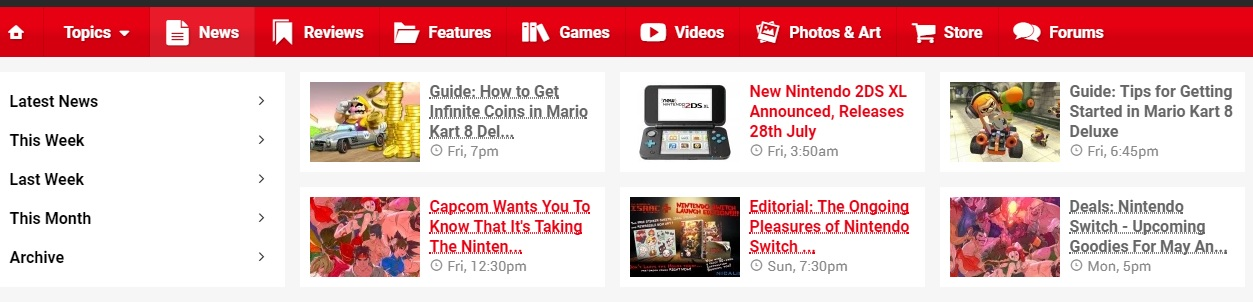
\includegraphics[width=\textwidth]{menu_nav}}
            \caption{\href{pic/menu_nav.jpg}{Menu a comparsa della sezione \emph{news}}\label{fig:menu-nav}}
        \end{figure}
    \end{itemize}
    \item Immediatamente sotto l'header è presente un banner pubblicitario
    \item Subito sotto c'è la \textbf{vetrina} con gli articoli principali del momento, e un altro banner pubblicitario a destra
    \item Sotto comincia la sezione con gli \textbf{articoli} ordinati in ``gruppi'' suddivisi per giorno di pubblicazione. In ogni gruppo gli articoli sono ordinati in modo cronologico secondo la seguente struttura:
    \begin{itemize}
        \item I 2 articoli più recenti sono ingranditi e affiancati.
        \item I successivi 4 articoli sono più piccoli e sono in sequenza verticale, e mostrano anche le prime parole del contenuto.
        \item I restanti sono ancora più piccoli e organizzati in griglia.
    \end{itemize}
    \item A destra della sezione articoli sono presenti vari contenuti consigliati, tra articoli e discussioni sul forum, e collegamenti ai canali social del sito.
    \item Sotto la sezione articoli, è presente una sezione con gli ultimi video pubblicati su \emph{Youtube}, un'altra con le ultime recensioni e, infine, una con le ultime foto postate dai redattori sul canale \emph{Instagram} del sito.
    \item Infine, nel \textbf{footer} e presente una barra di link per la ricerca di titoli che cominciano per una determinata lettera, una griglia contenente link agli articoli più popolari del momento, riferimenti ai profili del sito sui principali social network e link informativi sul sito.
\end{itemize}

\subsubsection{Analisi}
\label{sub:home-analisi}
Come prima impressione, la pagina è sicuramente \textbf{troppo lunga} \xmark: sono richiesti troppi \emph{scroll} per essere vista interamente. Sarebbe stato meglio spezzare il corpo del sito in più pagine (ad esempio, mostrare solo gli articoli e i contenuti di oggi).
Per quanto riguarda i 6 assi informativi, sono state fatte le seguenti osservazioni:
\begin{description}
    \item[Where] (\emph{dove siamo arrivati?}) \hfill \\ Nonostante non sia presente una breve descrizione del sito in cima alla pagina \xmark, è abbastanza chiaro già dal logo e dal nome del sito il contenuto dello stesso \cmark; inoltre, la presenza del pulsante di navigazione \emph{news} relativamente in alto a sinistra nella prima schermata fa intendere che il sito si occupi principalmente di notizie sul mondo Nintendo \cmark.
    \item[Who] (\emph{chi c'è dietro al sito?}) \hfill \\ Non c'è alcuna informazione a riguardo nella prima schermata che l'utente vede \xmark: le uniche informazioni sono presenti nel footer, a più di 10 scroll dall'inizio \xmark.
    \item[Why] (\emph{perché dovrei visitare il sito?}) \hfill \\ Questa domanda viene risposta in maniera implicita dai pulsanti di navigazione dell'header \cmark, che mostrano le varie tipologie di contenuti che il sito offre.
    \item[What] (\emph{che cosa offre il sito?}) \hfill \\  La vetrina è la risposta principale alla domanda \cmark; in misura minore, anche i tasti di navigazione (e i relativi menu a comparsa) mostrano l'offerta del sito \cmark.
    \item[When] (\emph{quali sono le ultime novità del sito?}) \hfill \\ Il pulsante \emph{news} è una delle prime cose che salta all'occhio \cmark; la vetrina riporta gli articoli più recenti e importanti \cmark; infine, la sezione articoli sottostante alla vetrina risponde perfettamente alla domanda \cmark, anche se richiede uno scroll per essere vista \xmark.
    \item[How] (\emph{come arrivo a ciò che mi interessa?}) \hfill \\ La barra di navigazione e i menu a comparsa sono molto efficaci \cmark; inoltre, per gli utenti registrati è possibile usare il menu \emph{hamburger} per arrivare più facilmente ai contenuti per loro interessanti \cmark.
\end{description}
Nel complesso l'utente, a una prima visita, dovrebbe essere in grado di capire facilmente che cosa offre il sito e come usufruirne \cmark.
Altre osservazioni:
\begin{itemize}
    \item[\cmark] Ogni articolo ha un \emph{blurb} che ancicipa brevemente il contenuto dello stesso
    \item[\cmark] Accanto al titolo di ogni articolo, è presente una \emph{keyword} (ben evidenziata) che ne definisce la tipologia (notizia, recensione, anteprima, video, curiosità, \ldots); questo aiuta l'utente a valutare se l'articolo è di suo interesse o meno
    \item[\cmark] L'header e la barra di navigazione compaiono in cima alla finestra se l'utente effettua uno scroll di una pagina verso l'alto; questo accorgimento mitiga il problema dell'eccessiva lunghezza della pagina, evitando all'utente di ritornare all'inizio per usare la barra di navigazione (questo comportamento accade in tutte le pagine del sito)
\end{itemize}
\clearpage
% !TEX encoding = UTF-8
% !TEX TS-program = pdflatex
% !TEX root = relazione.tex
% !TEX spellcheck = it-IT
\subsection{Pagina interna - Articolo}
\label{sub:articolo}
Anche in questo caso, le pagine degli articoli tendono a essere molto lunghe, per cui si consiglia di visualizzare il file \href{pic/articolo.jpeg}{\underline{articolo.jpeg}} (o di cliccare sull'immagine qui raffigurata).
\begin{figure}[h]
\centering
\href{pic/articolo.jpeg}{
\includegraphics[height=0.5\textheight]{articolo}}
\caption{\href{pic/articolo.jpeg}{Pagina interna - articolo}} % http://www.nintendolife.com/news/2017/05/nintendo_download_4th_may_europe
\end{figure}

\subsubsection{Struttura}
\label{sub:articolo-struttura}
Le pagine interne di articoli seguono tutte la stessa struttura, che è come segue:
\begin{itemize}
    \item \emph{Header} e \emph{Footer} identici a prima
    \item Sotto il primo banner pubblicitario, il contenuto comincia con una lista di \textbf{etichette} che denotano gli argomenti attinenti all'articolo corrente (ogni articolo ha delle etichette associate)
    \item Sotto il breadcrumb, viene ripreso il titolo e il \emph{blurb} visti anche nella homepage; è riportato inoltre il nome dell'autore dell'articolo, e a destra sono presenti pulsanti appositi per la condivisione su social network
    \item L'immagine immediatamente sotto è sempre presente (può essere rimpiazzata da un video) e generalmente è la versione completa della \emph{thumbnail} dell'articolo nella home
    \item Sotto comincia l'articolo vero e proprio
    \item Caso particolare di quest'articolo, è presente anche un sondaggio alla fine del testo
    \item Dopo il sondaggio c'è una lista di giochi correlati all'articolo
    \item Segue una griglia di banner pubblicitari che riprendono lo stile degli articoli nella homepage
    \item Dopo la pubblicità c'è la sezione commenti; in fondo alla lista è possibile, se registrati, inserire il proprio commento
    \item A sinistra della sezione commenti c'è una breve descrizione dell'autore e una lista di articoli correlati
    \item Nella sidebar a destra vi è una lista dei giochi menzionati nell'articolo che segue lo scroll della pagina.
\end{itemize}
Le recensioni dei giochi hanno due elementi aggiuntivi (fig.\ref{fig:recensione}): il voto assegnato al gioco e una ``finestra'' a destra che contiene le informazioni del titolo in esame. La finestra segue lo scroll dell'utente.
\begin{figure}[h]
    \centering
    \href{pic/recensione.jpeg}{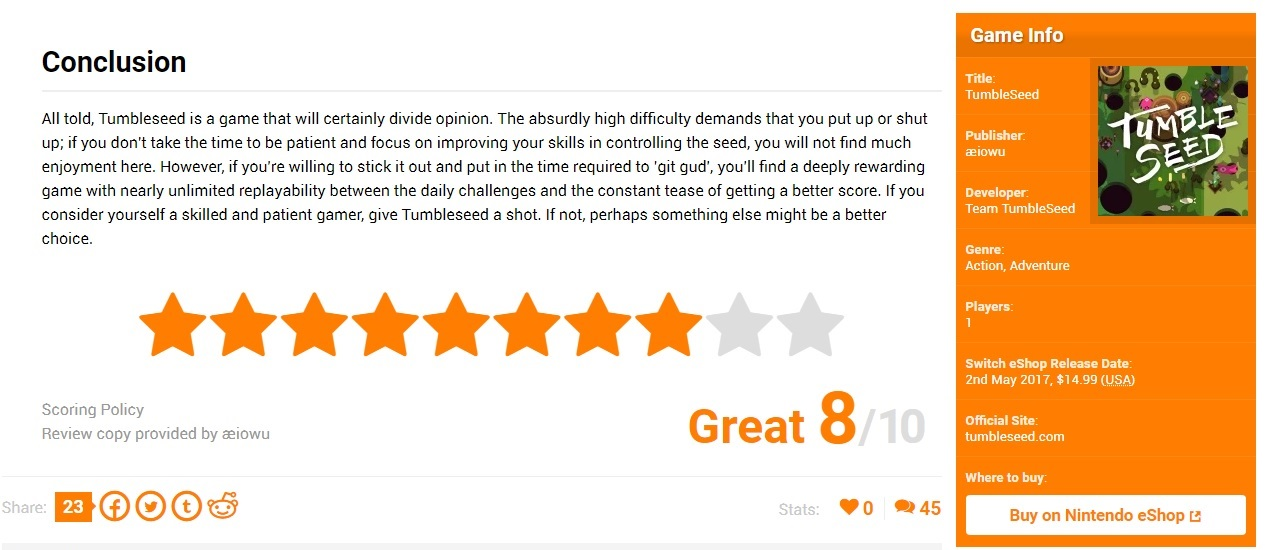
\includegraphics[width=\textwidth]{recensione}}
    \caption{\href{pic/recensione.jpeg}{Elementi aggiuntivi di una recensione}\label{fig:recensione}} % http://www.nintendolife.com/reviews/switch-eshop/tumbleseed#conclusion
\end{figure}

\subsubsection{Analisi}
\label{sub:articolo-analisi}
Anche in questo caso, la pagina rimane troppo lunga \xmark e il testo dell'articolo viene spinto troppo in basso dall'immagine: è probabile che l'utente sia costretto ad effettuare uno scroll per iniziare a leggerlo \xmark.\\
Essendo una pagina interna, non è necessario che tutti gli assi informativi siano sviluppati. Gli unici assi che rimangono obbligatori sono \textbf{Who} e \textbf{What}:
\begin{description}
    \item[Who] \hfill \\ Come nella homepage, le uniche informazioni a riguardo sono nel footer, quindi richiedono molto scroll per essere viste \xmark
    \item[What] \hfill \\ Rimane visibile la barra di navigazione, che mostra sinteticamente l'offerta del sito \cmark; inoltre, l'utente può passare sopra ai relativi pulsanti con il mouse per aprire i menu di navigazione, che forniscono ulteriori dettagli \cmark
\end{description}
Per quanto riguarda gli altri assi, sono state fatte le seguenti osservazioni:
\begin{description}
    \item[Where] \hfill \\ Poiché gli articoli non sono organizzati in una gerarchia, non ha senso utilizzare un breadcrumb per orientare l'utente: l'unico livello superiore nella gerarchia è sempre la homepage, accessibile cliccando il logo o l'icona relativa nella barra di navigazione \cmark; inoltre, la lista di etichette aiuta l'utente a capire a che tipologia di articolo è arrivato \cmark
    \item[Why] \hfill \\ I pulsanti della barra di navigazione continuano a mostrare all'utente che cosa offre il sito \cmark
    \item[When] \hfill \\ La lista degli articoli correlati mostra le notizie più recenti su argomenti analoghi alla pagina corrente \cmark
\end{description}

\section{Lista Immagini}
\label{sec:immagini}
%\listoffigures

\end{document}